\documentclass[17pt]{beamer}
%% 17pt gives quite big font, 20pt is massive!


\usepackage{url}
\usepackage{graphicx}
\usepackage{listings}
\lstset{basicstyle=\ttfamily,
  language=bash,
  showstringspaces=false
  keywordstyle=\color{red}
}

\begin{document}

\title{Intro to Linux}
\author{Jeremy Singer}

\frame{\titlepage}

\begin{frame}
  \frametitle{Teaser question}
  \begin{itemize}
  \item \visible<1->{How many two-letter words containing X are there ... for a game of scrabble?}
  \end{itemize}
 \visible<2->{
 \lstinputlisting{scrabble.sh}}
\end{frame}


\begin{frame}
\frametitle{Course objectives}
\begin{enumerate}
\item introduce Linux as a platform for developing software
\item gain experience with command line tools and scripting
\item encourage analysis of OS design and implementation
\end{enumerate}
\end{frame}

\begin{frame}
\frametitle{Learning sessions}
\begin{enumerate}
\item one-off Zoom with Q\&A (Mon 21 Sep, 12--1)
\item videos, worksheets and quizzes on Moodle
\item self-study labs (x3, Tue--Thu, 1--2)
\item labs with tutors (Tue 11--1, Tue 2--5, Wed 2--3, Thu 2--3, Fri 2--4)
\item no course assessment
\end{enumerate}
\end{frame}

% three surprising facts about Linux

\begin{frame}
\frametitle{Linux is everywhere}

From smartphones to supercomputers, from internet routers to Raspberry Pi

\begin{center}
  \includegraphics[width=3cm]{pi3.jpg}\hspace{10mm}%
  \includegraphics[width=5cm]{jeremy_in_datacenter.png}
\end{center}
\end{frame}


\begin{frame}
\frametitle{Linux is developed everywhere}

check out \url{www.remword.com/kps_result}
\begin{center}
  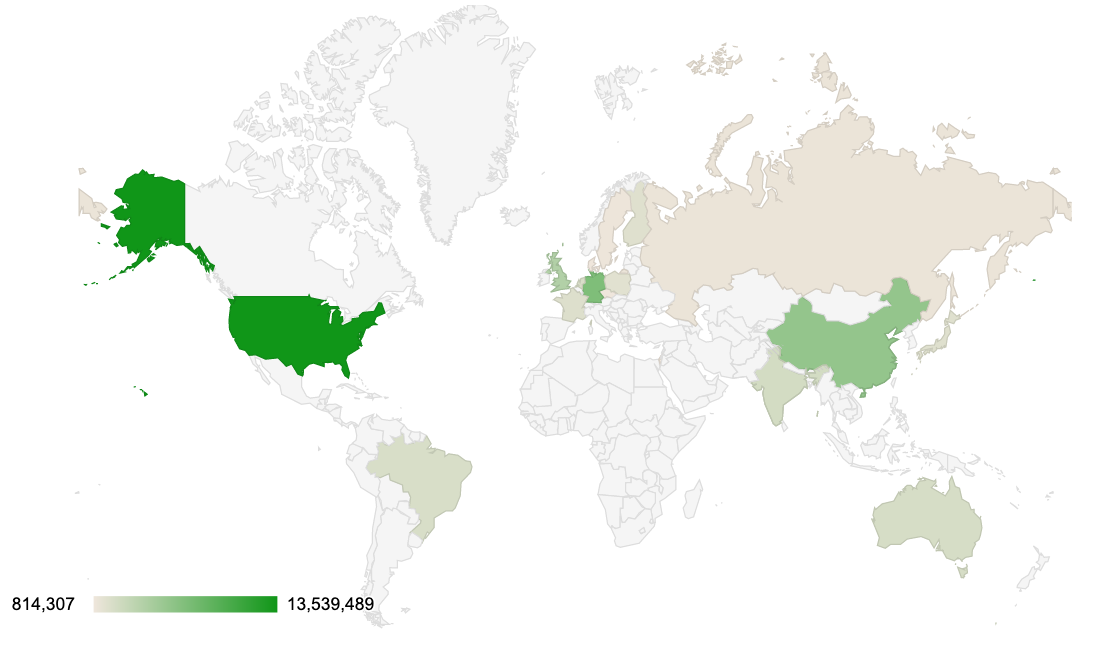
\includegraphics[width=\textwidth]{linux_world_map.png}
\end{center}

\end{frame}


\begin{frame}
\frametitle{Linux started as a one-person student project}
  {\tiny
    From: \url{torvalds@klaava.Helsinki.FI} (Linus Benedict Torvalds)
    Newsgroups: comp.os.minix
    Subject: What would you like to see most in minix?
    Summary: small poll for my new operating system
    Date: 25 Aug 91 20:57:08 GMT
    Organization: University of Helsinki

    Hello everybody out there using minix –

    I’m doing a (free) operating system (just a hobby, won’t be big and
    professional like gnu) for 386(486) AT clones. This has been brewing
    since april, and is starting to get ready. I’d like any feedback on
    things people like/dislike in minix, as my OS resembles it somewhat
    (same physical layout of the file-system (due to practical reasons)
    among other things).

    I’ve currently ported bash(1.08) and gcc(1.40), and things seem to work.
    This implies that I’ll get something practical within a few months, and
    I’d like to know what features most people would want. Any suggestions
    are welcome, but I won’t promise I’ll implement them :-)

    Linus 

    PS. Yes – it’s free of any minix code, and it has a multi-threaded fs.
    It is NOT protable (uses 386 task switching etc), and it probably never
    will support anything other than AT-harddisks, as that’s all I have :-(.

}
\end{frame}

\begin{frame}
  \frametitle{Next steps}

  \begin{itemize}
  \item Get access to a Linux terminal
  \item Start working through the materials on moodle
  \item Ask for help when you get stuck
  \end{itemize}
  
\end{frame}

\begin{frame}
  \frametitle{Buy my book!}

  \begin{center}
    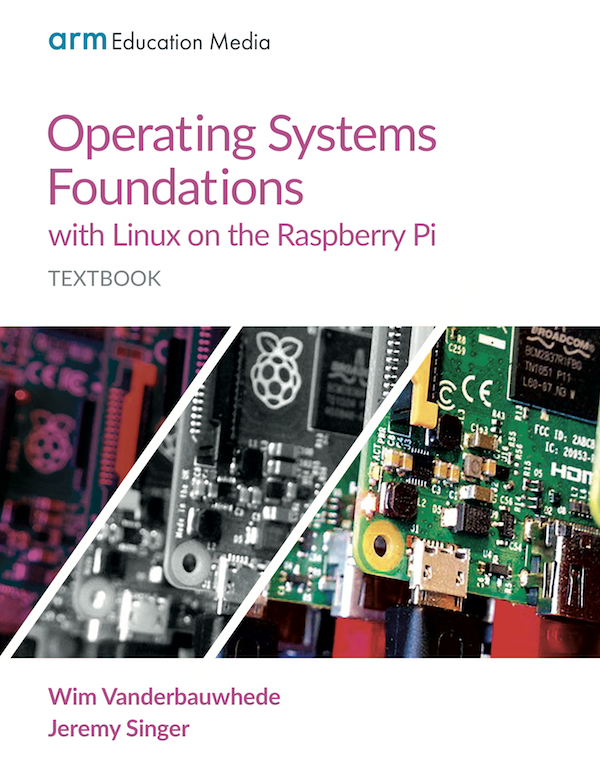
\includegraphics[width=5cm]{cover.png}
  \end{center}
  
\end{frame}

% useful information

%% \begin{frame}
%%   \frametitle{Useful info}
%%   \begin{itemize}
%%   \item login with your student id and last 8 digits of library barcode
%%   \item yell at me if you can't login
%%     \item fire up a terminal session --- \texttt{gnome-terminal} or similar
%%   \item access SoCS Linux remotely via server sibu.dcs.gla.ac.uk
%%   \end{itemize}
%% \end{frame}


\end{document}
